\documentclass[a4paper,9pt,twocolumn,twoside,]{pinp}

%% Some pieces required from the pandoc template
\providecommand{\tightlist}{%
  \setlength{\itemsep}{0pt}\setlength{\parskip}{0pt}}

% Use the lineno option to display guide line numbers if required.
% Note that the use of elements such as single-column equations
% may affect the guide line number alignment.

\usepackage[T1]{fontenc}
\usepackage[utf8]{inputenc}

% pinp change: the geometry package layout settings need to be set here, not in pinp.cls
\geometry{layoutsize={0.95588\paperwidth,0.98864\paperheight},%
  layouthoffset=0.02206\paperwidth, layoutvoffset=0.00568\paperheight}

\definecolor{pinpblue}{HTML}{185FAF}  % imagecolorpicker on blue for new R logo
\definecolor{pnasbluetext}{RGB}{101,0,0} %



\title{Creating a Kidney Transplant Risk Calculator using GEO datasets (Group
24)}

\author[]{460352996 470066919 480145820 480407614}

  \affil[]{GitHub code repository is
\href{https://github.sydney.edu.au/aauw2900/DATA3888FinalProject}{here}}

\setcounter{secnumdepth}{0}

% Please give the surname of the lead author for the running footer
\leadauthor{460352996 470066919 480145820 480407614}

% Keywords are not mandatory, but authors are strongly encouraged to provide them. If provided, please include two to five keywords, separated by the pipe symbol, e.g:
 \keywords{  Transplant |  Regression |  Prediction |  Immunosuppression  }  

\begin{abstract}
Background- Kidney failure is the final stage of renal disease and poses
a major threat to the body as the excretory system fails to function
properly. To combat kidney failure patients can choose two forms of
treatment in terms of medical intervention; renal dialysis or organ
transplantation. Renal dialysis is used to provide some kidney
functionalities by removing waste, maintaining a safe balance of
potassium, sodium and bicarbonate levels in the body and helps regulate
blood pressure (kidney dialysis). However, renal dialysis places several
restrictions on the patient, compromising their quality of life and is
not the ideal choice for patients with end stage kidney disease.
Alternatively, organ transplantation is a life saving treatment and is
greatly preferred over renal dialysis as it has the potential to offer a
better quality of life for the patient posing less restrictions on diet,
working lifestyle and posing fewer long term health problems. While
organ transplantation greatly preferred, kidney organ allocation has
posed itself as a major resource allocation problem. Donors and patients
need to be matched effectively and accurately to each other to not only
preserve the life of the patient but also, maximise functionality of
these limited kidney organs.
\end{abstract}

\dates{This version was compiled on \today} 

% initially we use doi so keep for backwards compatibility
% new name is doi_footer

\pinpfootercontents{A Research on Kidney Transplant}

\begin{document}

% Optional adjustment to line up main text (after abstract) of first page with line numbers, when using both lineno and twocolumn options.
% You should only change this length when you've finalised the article contents.
\verticaladjustment{-2pt}

\maketitle
\thispagestyle{firststyle}
\ifthenelse{\boolean{shortarticle}}{\ifthenelse{\boolean{singlecolumn}}{\abscontentformatted}{\abscontent}}{}

% If your first paragraph (i.e. with the \dropcap) contains a list environment (quote, quotation, theorem, definition, enumerate, itemize...), the line after the list may have some extra indentation. If this is the case, add \parshape=0 to the end of the list environment.


\hypertarget{aim-and-background}{%
\subsection{Aim and background}\label{aim-and-background}}

\hypertarget{aim-of-the-project}{%
\subsubsection{Aim of the project}\label{aim-of-the-project}}

With this problem in mind we developed a tool to aid in the effective
and accurate allocation of donor organs to their respective patients.
The developed risk calculator will assist practitioners in their
decision making and shall even inform the prescriptions for
immunosuppressive drugs. The risk calculator was developed with the
intention that it would be used in a clinical setting where shared
decision making is implemented. According to Gordan (2013), shared
decision making promotes patient centered care. It permits the
integration of the nephrologist's expertise on renal allograft
dysfunction with the patient's values and beliefs concerning future
treatment. Within this clinical setting, our hope would be that the risk
calculator provides an opportunity of discussion that concerns the
nature of treatment prior to, during and post organ transplantation.

\hypertarget{multidisciplinary-context}{%
\subsubsection{Multidisciplinary
context}\label{multidisciplinary-context}}

Changes being made\ldots{}\ldots{}

\hypertarget{target-audience}{%
\subsubsection{Target Audience}\label{target-audience}}

Should we have this here??????

\hypertarget{methods}{%
\subsection{Methods}\label{methods}}

\hypertarget{data-collection-and-developed-models}{%
\subsubsection{Data collection and developed
models}\label{data-collection-and-developed-models}}

\hypertarget{part-1.-predicting-acute-rejection}{%
\paragraph{Part 1. Predicting acute
rejection}\label{part-1.-predicting-acute-rejection}}

Acute Rejection (AR) calculator is based on data taken from the Gene
Expression Omnibus, GSE120396, GSE120649 and GSE131179. We merged the
three datasets together in order to achieve a larger sample size for
better accuracy, to identify outliers and provide a smaller margin of
error. However, because of the differences between datasets, such as
number of genes, scale (counts per million) and the use of ensembl ids
rather than gene ids, we have to perform some preprocessing before they
can be merged.

Inside the GSE120396, GSE120649 and GSE131179 folders are 88, 16 and 34
zipped files with file extension txt.gz respectively. Each of these
files has the gene expression count for one patient. They are unzipped
and placed together into a table format.

To resolve the issue of different units of measurements, we perform data
standardization. In particular, cpm and log2 transformation were
performed on GSE120649 and GSE131179. The ensemble id in GSE120649 and
GSE131179 were converted to gene symbols using the `EnsDb.Hsapiens.v79'
library from the Ensemble based annotation library from Bioconductor.

The three datasets were joined based on common gene symbols. To account
for any technical differences in gene expression measurements between
the three experiments, we perform quantile normalization. Quantile
normalization is one of the most widely adopted preprocessing methods
for analyzing microarray data. Quantile normalization reduces batch
effect and removes technological noise by scaling the variables to have
values between 0 and 1, ensuring the distribution of gene expressions
from each array are the same. This allowed more robust predictions that
can be generalised to different sequencing platforms (Qiu et.al, 2013).

From the high dimension of gene expression data between stable and acute
rejection patients, we performed feature selection using the `limma'
function to identify and extract the top 100 significant genes of the
kidney rejection dataset. These top 100 genes were used to build a
comprehensive model that can predict an acute re

Function to read in the files, unzip them, place them into a table

Preprocess data in the GSE Raw folder into a table, save it as a txt
file

\begin{Shaded}
\begin{Highlighting}[]
\NormalTok{gse_}\DecValTok{396}\NormalTok{ =}\StringTok{ }\KeywordTok{preprocessing_fn}\NormalTok{(}\StringTok{"../data/GSE120396_RAW/"}\NormalTok{)}
\KeywordTok{write.csv}\NormalTok{(gse_}\DecValTok{396}\NormalTok{, }\StringTok{"GSE120396_expression_matrix.txt"}\NormalTok{)}
\end{Highlighting}
\end{Shaded}

Install the Ensembl based annotation library from Bioconductor Function
takes a GSE table as input, and returns a GSE dataframe with two new
columns, `gene symbols' and `gene ids', from the `ensembl ids' using the
library above.

\begin{Shaded}
\begin{Highlighting}[]
\KeywordTok{library}\NormalTok{(}\StringTok{"EnsDb.Hsapiens.v79"}\NormalTok{)}

\NormalTok{emsembl_to_symbol <-}\StringTok{ }\ControlFlowTok{function}\NormalTok{(gse) \{}
\NormalTok{    G_list <-}\StringTok{ }\KeywordTok{select}\NormalTok{(EnsDb.Hsapiens.v79, }
        \DataTypeTok{key =} \KeywordTok{rownames}\NormalTok{(gse), }
        \DataTypeTok{columns =} \KeywordTok{c}\NormalTok{(}\StringTok{"SYMBOL"}\NormalTok{), }
        \DataTypeTok{keytype =} \StringTok{"GENEID"}\NormalTok{)}
\NormalTok{    df =}\StringTok{ }\KeywordTok{as.data.frame}\NormalTok{(gse)}
\NormalTok{    df_symbol <-}\StringTok{ }\KeywordTok{merge}\NormalTok{(df, }
\NormalTok{        G_list, }\DataTypeTok{by.x =} \DecValTok{0}\NormalTok{, }
        \DataTypeTok{by.y =} \StringTok{"GENEID"}\NormalTok{, }
        \DataTypeTok{all.x =} \OtherTok{TRUE}\NormalTok{)}
    \KeywordTok{return}\NormalTok{(df_symbol)}
\NormalTok{\}}
\end{Highlighting}
\end{Shaded}

Log the two datasets, 649 and 179, and use the ensembl function to get
the gene symbols for both datasets. Finally, merge the datasets by gene
symbols.

\begin{Shaded}
\begin{Highlighting}[]
\CommentTok{# log 649!}
\NormalTok{log_}\DecValTok{649}\NormalTok{ <-}\StringTok{ }\KeywordTok{log2}\NormalTok{(gse_}\DecValTok{649}\NormalTok{)}
\NormalTok{log_}\DecValTok{649}\NormalTok{[log_}\DecValTok{649} \OperatorTok{==}\StringTok{ }\OperatorTok{-}\OtherTok{Inf}\NormalTok{] <-}\StringTok{ }\DecValTok{0}
\NormalTok{df_}\DecValTok{649}\NormalTok{_symbol =}\StringTok{ }\KeywordTok{emsembl_to_symbol}\NormalTok{(log_}\DecValTok{649}\NormalTok{)}

\CommentTok{# 179!}
\NormalTok{log_}\DecValTok{179}\NormalTok{ <-}\StringTok{ }\KeywordTok{log2}\NormalTok{(gse_}\DecValTok{179}\NormalTok{)}
\NormalTok{log_}\DecValTok{179}\NormalTok{[log_}\DecValTok{179} \OperatorTok{==}\StringTok{ }\OperatorTok{-}\OtherTok{Inf}\NormalTok{] <-}\StringTok{ }\DecValTok{0}
\NormalTok{df_}\DecValTok{179}\NormalTok{_symbol =}\StringTok{ }\KeywordTok{emsembl_to_symbol}\NormalTok{(log_}\DecValTok{179}\NormalTok{)}

\CommentTok{# left join both}
\NormalTok{df_both <-}\StringTok{ }\KeywordTok{merge}\NormalTok{(df_}\DecValTok{179}\NormalTok{_symbol, }
\NormalTok{    df_}\DecValTok{649}\NormalTok{_symbol, }\DataTypeTok{by.x =} \StringTok{"Row.names"}\NormalTok{, }
    \DataTypeTok{by.y =} \StringTok{"Row.names"}\NormalTok{, }
    \DataTypeTok{all.x =} \OtherTok{TRUE}\NormalTok{)}
\NormalTok{df_both}
\end{Highlighting}
\end{Shaded}

We plot the distribution of patient gene expression measurements using a
boxplot to see if we have to remove any patient that has measurements
unlike the others.

\begin{Shaded}
\begin{Highlighting}[]
\NormalTok{p <-}\StringTok{ }\KeywordTok{ggplot}\NormalTok{(}\KeywordTok{melt}\NormalTok{(gse_}\DecValTok{396}\NormalTok{), }
    \KeywordTok{aes}\NormalTok{(}\DataTypeTok{x =}\NormalTok{ Var2, }\DataTypeTok{y =}\NormalTok{ value)) }\OperatorTok{+}\StringTok{ }
\StringTok{    }\KeywordTok{geom_boxplot}\NormalTok{(}\DataTypeTok{outlier.colour =} \StringTok{"black"}\NormalTok{, }
        \DataTypeTok{outlier.shape =} \DecValTok{16}\NormalTok{, }
        \DataTypeTok{outlier.size =} \FloatTok{0.5}\NormalTok{, }
        \DataTypeTok{notch =} \OtherTok{FALSE}\NormalTok{) }\OperatorTok{+}\StringTok{ }
\StringTok{    }\KeywordTok{theme}\NormalTok{(}\DataTypeTok{axis.text.x =} \KeywordTok{element_text}\NormalTok{(}\DataTypeTok{angle =} \DecValTok{45}\NormalTok{, }
        \DataTypeTok{hjust =} \DecValTok{1}\NormalTok{)) }\OperatorTok{+}\StringTok{ }
\StringTok{    }\KeywordTok{labs}\NormalTok{(}\DataTypeTok{x =} \StringTok{"patient"}\NormalTok{, }
        \DataTypeTok{y =} \StringTok{"expression value"}\NormalTok{) }\OperatorTok{+}\StringTok{ }
\StringTok{    }\KeywordTok{theme_minimal}\NormalTok{()}
\NormalTok{p}
\end{Highlighting}
\end{Shaded}

\hypertarget{part-2.-estimating-time-to-de-novo-dsa-presence}{%
\paragraph{Part 2. Estimating Time to de novo DSA
Presence}\label{part-2.-estimating-time-to-de-novo-dsa-presence}}

The data and data dictionary used were provided by Dr.~Jermaine wong.

Certain columns in the data were mutated as follows. 0 and 1 variables
in the Sex\_Cat columns were mapped to FEmale and Male respectively. The
values in the agetxn columns were rounded and grouped into 3 categories
`25-35','36-45', and `46-55'. C2epletMM were also grouped into
categories,'\textless{}= 30 MM' and ` \textgreater{} = 30MM'.

Here we first create a survival object using the Surv() function, to
which we feed in the ``C2dnDSA'', ``C2daystodnDSA'' information, which
in turn is used as the dependent variable for the Kaplan-Meier Formula.
The data set is filtered by the selected user input(Age group and
Gender) and passed in as the Independent variable. We plot the Kaplan
Meier Curve using the survfit() function.

Based on previous research studies conducted it was found that there was
no significant correlation between BMI category and graft survival
(Papalia et.al, 2010) Thus we focused on only using age and gender as
phenotypic information when stratifying the data to fit a particular
recipient.

\hypertarget{part-3.-predicting-operational-tolerance}{%
\paragraph{Part 3. Predicting Operational
Tolerance}\label{part-3.-predicting-operational-tolerance}}

To predict operational tolerance, we collected the GSE22229 dataset that
contained raw gene expressions from tolerant patients and normal
patients (which still required immune suppression for stable graft
function). GSE22229 dataset was a raw CEL dataset containing 58 zipped
files, each pertaining to the gene expression for one patient that was
either tolerant (19), undergoing normal immunosuppression (27), or
standard controls (12). In this case, we only retained the tolerant and
immunosuppressed patients for our analysis.

CEL files are data files created by the Affymetrix DNA microarray image
analysis software, and contain estimated probe (sequence of DNA base
pairs) intensity values extracted from biological chips called
Affymetrix Genechips. Each probe was mapped to a specific gene symbol
using the GPL570 Chip Description File (CDF).

Since the data is in the newer Affymetrix Arrays format (Gene ST
arrays), we utilised the `oligo' library and its functions,
`list.celfiles' and `read.celfiles', to read a list of CEL files into
our directory. This list was then converted from an AffyBatch object
into an ExpressionSet (i.e.~gene expression) using the `rma' function
from the `pd.mogene.2.0.st' library. The `rma' function, short for
Robust Multichip Average, also simultaneously log2 transforms and
normalises the gene expressions.

After converting our ExpressionSet object into a dataframe, we then
investigated the gene expression distribution amongst patients using a
boxplot to ensure that the data has been normalised and can be used for
further processing.

The boxplot above demonstrates strong similarity in gene expression
between patients and so our dataframe can be further analysed without
concern of batch effects between sample measurements.

After quantile normalization and batch effect removal, we performed
feature selection. Firstly, genes that were lowly expressed in both
groups were removed by using the filterByExpr() function from the edgeR
package; these genes do not provide much biological meaning and removing
them allows for less statistical tests to be performed, as well as
allowing greater reliability in observing the variance between different
groups (Law et al., 2018).

We then selected the top 100 most differentially expressed genes between
the two groups using multiple t-tests from the \texttt{limma} package.
Finally, a review by Massart et al. (2017) suggested a collection of
genes that were highly differential between tolerant and normal
patients, and so these were also added to our final training dataset (if
they weren't already filtered for previously).

Installing essential tac packages

\begin{Shaded}
\begin{Highlighting}[]
\KeywordTok{library}\NormalTok{(limma)}
\KeywordTok{library}\NormalTok{(affy)}
\KeywordTok{library}\NormalTok{(oligo)}
\KeywordTok{library}\NormalTok{(pd.mogene.}\DecValTok{2}\NormalTok{.}\FloatTok{0.}\NormalTok{st)}
\KeywordTok{library}\NormalTok{(mogene20sttranscriptcluster.db)}
\KeywordTok{library}\NormalTok{(GEOquery)}
\end{Highlighting}
\end{Shaded}

\begin{Shaded}
\begin{Highlighting}[]
\KeywordTok{setwd}\NormalTok{(}\StringTok{"data/GSE22229_RAW/"}\NormalTok{)}
\NormalTok{celFiles <-}\StringTok{ }\KeywordTok{list.celfiles}\NormalTok{()}
\NormalTok{affyRaw <-}\StringTok{ }\KeywordTok{read.celfiles}\NormalTok{(celFiles)}
\NormalTok{eset <-}\StringTok{ }\KeywordTok{rma}\NormalTok{(affyRaw)}

\KeywordTok{setwd}\NormalTok{(}\StringTok{"../../"}\NormalTok{)}
\KeywordTok{write.exprs}\NormalTok{(eset, }\DataTypeTok{file =} \StringTok{"tolerance.txt"}\NormalTok{)}
\NormalTok{my_frame <-}\StringTok{ }\KeywordTok{data.frame}\NormalTok{(}\KeywordTok{exprs}\NormalTok{(eset))}
\KeywordTok{write.table}\NormalTok{(my_frame, }
    \DataTypeTok{file =} \StringTok{"tolerance.txt"}\NormalTok{, }
    \DataTypeTok{sep =} \StringTok{"}\CharTok{\textbackslash{}t}\StringTok{"}\NormalTok{)}
\end{Highlighting}
\end{Shaded}

\hypertarget{evaluation-strategies}{%
\subsubsection{Evaluation Strategies}\label{evaluation-strategies}}

We decided to implement penalised logistic regression methods when
creating a predictive model for Part 1 and Part 3 of our risk
calculator. Logistic regression was utilised as it provides a
probabilistic output for a specific risk, which may be more informative
than a binary outcome. Furthermore, the penalised nature of some methods
(e.g.~Ridge, LASSO, Elastic Net) can address the overfitting or
multicollinearity issue prevalent in large p, small n situations
prevalent in gene expression data.

For Part 1 and Part 3 respectively, our model was trained using a
50-repeated 5-fold cross validation (CV) procedure. The performance of
our model in predicting the CV test-set under Ridge, LASSO and Elastic
Net methods were evaluated using three primary metrics: accuracy, AUC
and the Brier Score.

In the case of class imbalance within the training dataset, the accuracy
metric may suggest an inflated performance. As such, the AUC and Brier
Score were also calculated.

\begin{itemize}
\item
  The AUC is a more robust metric with less bias to class size. Briefly,
  it can be thought of as the probability that a true-positive sample
  (e.g.~AR patient) has a greater predicted risk than true-negative
  samples (e.g.~normal patient).
\item
  The Brier Score meanwhile complements the AUC by checking that the
  predicted risk of a sample is actually similar to the true value. For
  example, in a true-positive case (i.e.~label = 1) with a predicted
  risk of 0.8, the Brier Score quantitatively measures how close the 0.8
  value is to 1. Better predictions are reflected as a lower Brier
  Score.
\end{itemize}

To select our final models for Part 1 and Part 3 respectively, we
quantitatively compared the accuracy, AUC and Brier Score from different
penalised models (Ridge, LASSO, and Elastic Net) using boxplot
visualisations.

We also evaluate the model based on robustness. Robustness refers to how
well the model achieves its aim when it is applied to the general
population, which is our target audience. We qualitatively analysed
robustness by estimating how well the model will adjust if it is applied
to real-world data, which may have potential issues such as missing
information.This evaluation metric ensures the external validity of the
product.

\hypertarget{results}{%
\subsection{Results}\label{results}}

\hypertarget{final-model}{%
\subsubsection{Final Model}\label{final-model}}

\hypertarget{deployment-process}{%
\subsubsection{Deployment Process}\label{deployment-process}}

\hypertarget{discussion-and-conclusion}{%
\subsection{Discussion and Conclusion}\label{discussion-and-conclusion}}

\hypertarget{potential-shortcomings}{%
\subsubsection{Potential shortcomings}\label{potential-shortcomings}}

\hypertarget{future-work-and-improvements}{%
\subsubsection{Future work and
improvements}\label{future-work-and-improvements}}

\hypertarget{conclusion}{%
\subsubsection{Conclusion}\label{conclusion}}

\newpage

\hypertarget{reference-list}{%
\subsection{Reference List}\label{reference-list}}

\hypertarget{section}{%
\subsubsection{1.}\label{section}}

Dayoub, J.C. Cortese, F., Anzic, A, 2018, The Effects of Donor Age on
Organ transplants: a review and implications for aging research,
Experimental Gerontology, Vol 110, pp.~230-240, Retrieved from
\textless{}\textgreater{}

\hypertarget{section-1}{%
\subsubsection{2.}\label{section-1}}

Dorr, C. R., Oetting, W. S., Jacobson, P. A., \& Israni, A. K. (2018).
Genetics of acute rejection after kidney transplantation. Transplant
International, 31(3), 263-277.

\hypertarget{section-2}{%
\subsubsection{3.}\label{section-2}}

Edgar R., Domrachev M., Lash AE. (2002). Gene Expression Omnibus: NCBI
gene expression and hybridization array data repository. Nucleic Acids
Res, 30(1),207-10.

\hypertarget{section-3}{%
\subsubsection{4.}\label{section-3}}

Gordon, E.J., 2013, Opportunities for Shared Decision Making in Kidney
Transplantation, American Journal of Transplantation, Vol.13, no.5
pp.~1149-1158.

\hypertarget{section-4}{%
\subsubsection{5.}\label{section-4}}

Kleinbaum, D.G., 2005 Klein, M., `Introduction to Survival Analaysis' in
Survival Analysis: A self learning text, Springer, New York, NY pp.1-43.

\hypertarget{section-5}{%
\subsubsection{6.}\label{section-5}}

Massart, A., Ghisdal, L., Abramowicz, M., \& Abramowicz, D. (2017).
Operational tolerance in kidney transplantation and associated
biomarkers. Clinical \& Experimental Immunology, 189(2), 138-157.

\hypertarget{section-6}{%
\subsubsection{7.}\label{section-6}}

Tambur, A.R. 2018, HLA-epitope Matching or Eplet Risk Stratification:
The Devil is in the Details, Front Immunol, Vol.9

\hypertarget{appendixes}{%
\subsection{Appendixes}\label{appendixes}}

\hypertarget{appendix-a}{%
\subsubsection{Appendix A}\label{appendix-a}}

Kaplan-Meier curve: Estimated Probability for Class II de novo DSA
Appearance

\begin{center}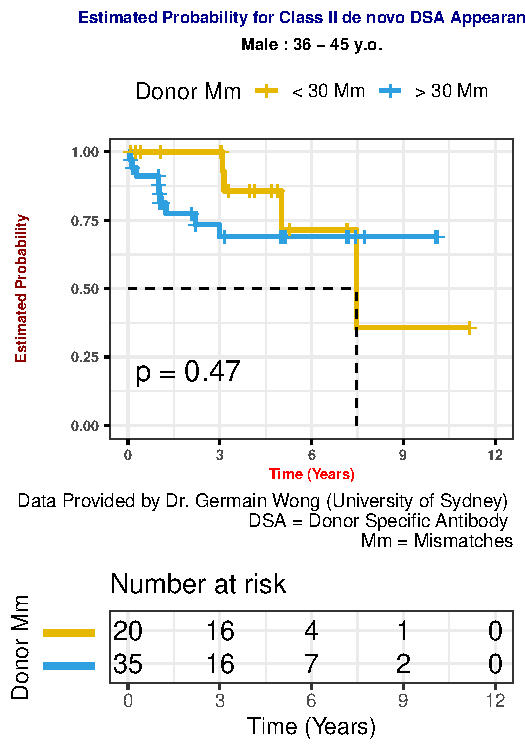
\includegraphics{Executive_Report_files/figure-latex/eplet-1} \end{center}

\hypertarget{appendix-b}{%
\subsubsection{Appendix B}\label{appendix-b}}

Penalised Logistic Regression: Risk of Acute Rejection

\hypertarget{appendix-c}{%
\subsubsection{Appendix C}\label{appendix-c}}

Penalised Logistic Regression: Reliance on Immunosuppression

\hypertarget{contribution-statement}{%
\subsection{Contribution Statement}\label{contribution-statement}}

\hypertarget{johanna-jones}{%
\subsubsection{Johanna Jones}\label{johanna-jones}}

\hypertarget{andrew-auwyang}{%
\subsubsection{Andrew Auwyang}\label{andrew-auwyang}}

\hypertarget{eva-pu}{%
\subsubsection{Eva Pu}\label{eva-pu}}

\hypertarget{niruth-bogahawatta}{%
\subsubsection{Niruth Bogahawatta}\label{niruth-bogahawatta}}

\hypertarget{alex-wong}{%
\subsubsection{Alex Wong}\label{alex-wong}}

%\showmatmethods


\bibliography{pinp}
\bibliographystyle{jss}



\end{document}

